\section{Projektadministration}
Til at holde overblik over opgaver blev programmet Zenhub brugt. Dette er en add-on til Github, som var vores versionsstyringsværktøj. \\
Zenhub gjorde det muligt at have et elektronisk scrum-board, hvor alle opgaver blev oprettet så begge gruppe medlemmer havde et overblik over hvad der manglede og hvad man arbejde med lige nu. \\
Et skærmbillde af scrum boardet i zenhub kan ses på figur \ref{fig:ZenhubScrum}.

\begin{figure} [H]
	\begin{center}
		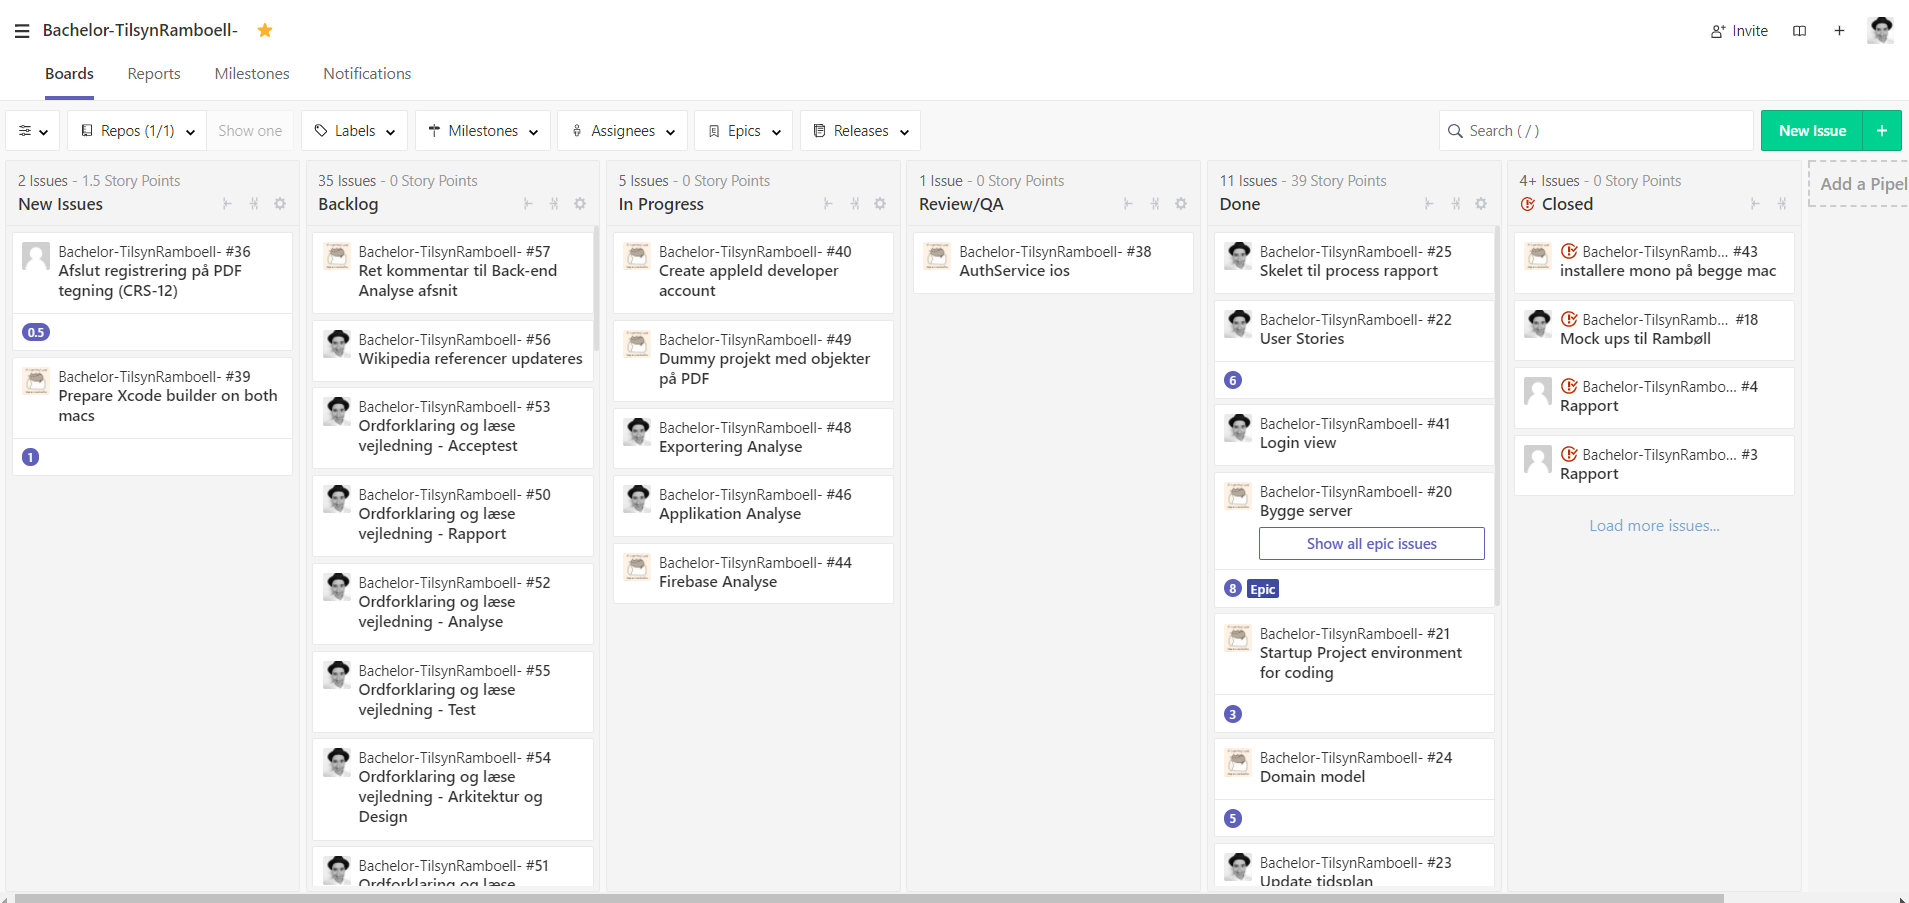
\includegraphics[height=8cm, width=15cm]{Projektadministration/Zenhub}
	\end{center}
	\caption{Scrum-board i Zenhub}
	\label{fig:ZenhubScrum}
\end{figure} 
